\subsection{Requerimientos no funcionales}
\subsubsection{Plataforma}
\begin{itemize}
    \item {Sistema gestor de bases de datos: MySQL Server  versión 5.0}
    \item {Lenguaje de programación de propósito general: PHP versión 7.0}
    \item {Navegador web: Cualesquiera de las versiones de Google Chrome, Mozilla Firefox y/o Safari}
    \item {Memoria de Acceso Aleatorio: 4GB mínimo, 8GB recomendado}
    \item {Procesador: Cuatro núcleos a 2.4GHz (recomendado)}
\end{itemize}

En el diagrama de despliegue~\ref{fig:plataforma} podemos visualizar exactamente las mismas especificaciones.
\begin{figure}[H]
    \centering
    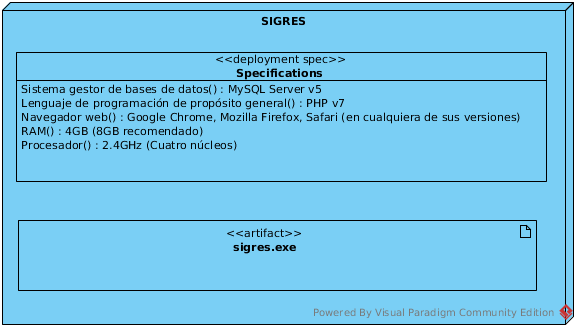
\includegraphics[scale=.7]{images/plataforma.png}
    \centering
    \caption{DRNF01: Plataforma del sistema.}
    \label{fig:plataforma}
\end{figure}

\subsubsection{Interacción del Usuario}
\begin{itemize}
    \item {}
\end{itemize}

\subsubsection{Procesos del negocio}
En la siguiente tabla~\ref{tbl:listaUP} se muestran los usuarios contemplados para el diseño del sistema y los procesos que se modelaron.
\begin{longtable}[H]{m{4cm}m{8cm}}
    \toprule
    \centering \textbf{Usuario} & \centering  \textbf{Procesos} \tabularnewline
    \midrule
    \textbf{Gerente de Ventas} & Alta de un nuevo cliente, cambios a un cliente existente, búsqueda de un cliente, visualización datos de todo el listado de clientes, eliminación de datos de un cliente perdido.\tabularnewline
    \textbf{Agente de ventas} & Alta de un nuevo cliente, cambios a un cliente existente, búsqueda de un cliente, visualización datos de todo el listado de clientes.\tabularnewline
    \textbf{Titular de Jurídico} & Alta de un nuevo permiso (cualesquiera de los tres emitidos por: Secretaría de Seguridad Pública de la Ciudad de México, Secretaría de Obras y Servicios de la Ciudad de México, Secretaría de Protección Civil de la Ciudad de México), cambios a un permiso registrado (cualesquiera de los tres emitidos por: Secretaría de Seguridad Pública de la Ciudad de México, Secretaría de Obras y Servicios de la Ciudad de México, Secretaría de Protección Civil de la Ciudad de México), búsqueda de un permiso registradi (cualesquiera de los tres emitidos por: Secretaría de Seguridad Pública de la Ciudad de México, Secretaría de Obras y Servicios de la Ciudad de México, Secretaría de Protección Civil de la Ciudad de México), visualización datos de todo el listado de permisos vigentes asociado a un espectacular, alta de una nueva póliza de seguros de un espectacular, cambios  a una póliza de seguros de un espectacular,  visualización datos de póliza de seguros vigente asociada a un espectacular, eliminación de datos de una póliza de seguros, eliminación de datos de un permiso cualesquiera de los tres emitidos por: Secretaría de Seguridad Pública de la Ciudad de México, Secretaría de Obras y Servicios de la Ciudad de México, Secretaría de Protección Civil de la Ciudad de México).\tabularnewline
    \textbf{Agente jurídico} & Alta de un nuevo permiso (cualesquiera de los tres emitidos por: Secretaría de Seguridad Pública de la Ciudad de México, Secretaría de Obras y Servicios de la Ciudad de México, Secretaría de Protección Civil de la Ciudad de México), cambios a un permiso registrado (cualesquiera de los tres emitidos por: Secretaría de Seguridad Pública de la Ciudad de México, Secretaría de Obras y Servicios de la Ciudad de México, Secretaría de Protección Civil de la Ciudad de México), búsqueda de un permiso registradi (cualesquiera de los tres emitidos por: Secretaría de Seguridad Pública de la Ciudad de México, Secretaría de Obras y Servicios de la Ciudad de México, Secretaría de Protección Civil de la Ciudad de México), visualización datos de todo el listado de permisos vigentes asociado a un espectacular, alta de una nueva póliza de seguros de un espectacular, cambios  a una póliza de seguros de un espectacular,  visualización datos de póliza de seguros vigente asociada a un espectacular.\tabularnewline
    \textbf{Jefe de Infraestructura} & Alta de un nuevo espectacular, cambios a un espectacular existente, búsqueda de un espectacular, visualización datos de todo el listado de espectaculares, eliminación de un espectacular.\tabularnewline
    \textbf{Agente de Infraestructura} & Alta de un nuevo espectacular, cambios a un espectacular existente, búsqueda de un espectacular, visualización datos de todo el listado de espectaculares.\tabularnewline
    \textbf{Jefe de Capital Humano} & Alta de un nuevo empleado, cambios a un empleado existente, visualización datos de todo el listado de empleados, eliminación de un empleado.\tabularnewline
    \textbf{Agente de Capital Humano} & Alta de un nuevo empleado, cambios a un empleado existente, visualización datos de todo el listado de empleados. \tabularnewline

\caption{Usuarios y procesos contemplados}
\label{tbl:listaUP}
\bottomrule
<<<<<<< HEAD
\end{longtable}
=======
\end{longtable}
>>>>>>> master


\subsubsection{Información y datos}

\subsubsection{Propiedades del software}
\begin{itemize}
    \item Verificabilidad
    \item Correctitud
    \item Confiabilidad
    \item Amigabilidad
    \item Mantenibilidad
    \item Reparabilidad
    \item Evolucionabilidad
\end{itemize}
